% STALA 2027 submission (double-blind). NDSS 2027 template (IEEEtran.cls
% from the NDSS 2027 templates page). Build: latexmk -pdf main.tex
% Numbers come from the README and docs/paper/*.md; see SOURCES.md.
\documentclass[conference]{IEEEtran}
\usepackage[T1]{fontenc}
\usepackage{times}
\usepackage{graphicx}
\usepackage{booktabs}
\usepackage{url}
\usepackage{xspace}
\usepackage{amsmath}
\usepackage[hidelinks]{hyperref}
\graphicspath{{../figures/}}
\setlength{\emergencystretch}{1.5em}
\pagestyle{plain}

\newcommand{\takapay}{TakaPay\xspace}
\newcommand{\prov}{\texttt{provenance}\xspace}
\newcommand{\provamt}{\texttt{provenance-amount}\xspace}
\newcommand{\provcon}{\texttt{provenance-consistent}\xspace}
\newcommand{\repourl}{\url{https://anonymous.4open.science/r/takapay-bench}}

\begin{document}

\title{Bangla Is Not a Shield: Testing Prompt-Injection\\Defences for Mobile-Money Agents}

\author{\IEEEauthorblockN{Anonymous submission}}

\IEEEoverridecommandlockouts
\makeatletter\def\@IEEEpubidpullup{6.5\baselineskip}\makeatother
\IEEEpubid{\parbox{\columnwidth}{
    Workshop on Security Testing and Assurance for LLMs and Agents (STALA) 2027\\
    22 March 2027, Seoul, Republic of Korea\\
    ISBN 978-1-970672-xx-x\\
    https://dx.doi.org/10.14722/stala.2027.xxxxx\\
    www.ndss-symposium.org
}
\hspace{\columnsep}\makebox[\columnwidth]{}}

\maketitle

\begin{abstract}
LLM agents that read messages and make payments are arriving in mobile
money, where users and scammers write in Bangla, romanised Bangla
(Banglish) and code-mixed text. We release \takapay, a benchmark of 302
cases in which indirect prompt injections hidden in SMS, invoices and tool
descriptions try to make an agent pay an attacker, leak a one-time code or
overpay the real payee, and test six models from three families. No
injection detector we tested both caught the attacks and let Bangla
payments through: an English-trained one flagged 84\% of normal Bangla
texts, the multilingual Prompt Guard~2 flagged none of the 174 attacks,
and a policy model given a policy written for these attacks caught 93\%
but blocked real family payment requests and missed every amount-only
attack. Attacks in Bangla worked less often than in English, but only on
models that also handled Bangla requests poorly; on a model fluent in all
four languages they worked equally well, so a low-resource language is not
a lasting shield. We also report testing lessons: attack success alone
hides wrong payments made with no attacker and can hinge on one template,
checking only whether the attacker was paid misses amount-only attacks,
and harness details and scripted audits change the conclusions.
\end{abstract}

\IEEEpeerreviewmaketitle

% ---------------------------------------------------------------------
\section{Introduction}

Bangladesh has 239 million mobile money (MFS) users~\cite{bangladeshbank2025mfs},
and fraud by impersonation and PIN or one-time code (OTP) theft is
common. AI assistants that read a user's messages and pay for them are
arriving, and the top risk in the OWASP Top~10 for Agentic
Applications~\cite{owasp2026agentic}, agent goal hijack, is mostly delivered
by indirect prompt injection~\cite{greshake2023indirect}: instructions hidden
in content the agent reads. For a payment agent that content is the inbox
and the bills, written in Bangla script, in romanised Bangla (Banglish)
with no fixed spelling, and in text that switches language inside a
sentence.

Agent prompt-injection benchmarks such as InjecAgent~\cite{zhan2024injecagent}
and AgentDojo~\cite{debenedetti2024agentdojo} are in English. Multilingual
safety work, including work on Bengali~\cite{deng2024multijail,wang2024xsafety,islam2026banglasafe},
studies jailbreaks of chat models, where the harm is text; Bangla
prompt-injection work so far trains detectors on machine-translated
text~\cite{muhtadi2026mipiad}, and a case study covers Tamil and Tanglish on
one model~\cite{g2026tanglish}. None runs agents whose harm is an action. We
ask whether attacks, and the defences built against them, carry over to an
agent that moves money in Bangla.

\textbf{Detectors flag the script or miss the attack.} We ran five
injection detectors on every untrusted text in the benchmark. ProtectAI's
English-trained classifier flagged 16 of 19 normal Bangla texts (84\%), such
as a power bill and a mother asking for medicine money, more often than
Bangla attacks (57\%); as a filter it would break 20 of 22 normal tasks
requested in Bangla and 1 of 21 in English. Meta's multilingual Prompt
Guard~2 flagged no normal text, and none of the 174 attacks. gpt-oss-safeguard,
given a policy we wrote for these attacks, caught 93\% in every language
but flagged family requests for money and missed every attack that only
raises a bill's amount.

\textbf{What worked instead.} Provenance checks where a payment's
recipient, code and amount came from, never what the text says. The idea
is not ours: CaMeL~\cite{debenedetti2025camel} and information-flow control
such as FIDES~\cite{costa2025fides} enforce it, evaluated in English. We
test a deliberately simple rule-based version at the tool boundary on six
models (Qwen2.5 3B to 32B, Hermes~3 on Llama~3.1 8B, GPT-OSS-120B). Its
decisions do not depend on the language, so neither does its cost. Which
attacks such rules stop follows from their design, so we report those as
rule properties, verified by replaying every recorded call, and use the
runs for what agents attempt and what the rules cost.

\textbf{Testing lessons.} The runs also show how easily a payment-agent
benchmark misleads. (i)~\emph{Attack success alone misleads}: with no
attacker, the Qwen models tried to pay a payee or amount nobody asked for
in 29\% to 52\% of episodes, more often than any attack succeeded, while
GPT-OSS-120B's 15.0\% attack success came almost entirely from one
template. (ii)~\emph{Bangla is not a shield}: three Qwen models followed
English attacks far more than Bangla ones but also completed far fewer
Bangla requests; GPT-OSS-120B handled all four languages and attacks worked
equally in all four. (iii)~\emph{``Was the attacker paid?'' misses
amount-only attacks}, which keep the real payee and raise the amount.
(iv)~\emph{Harness and audit change the conclusions}: rewording one block
message brought back 12 normal tasks for one model, and a scripted audit
reported a defence as complete until a real model, reading only the newest
SMS, got past it.

\textbf{Contributions.} (1)~\takapay, a fictional mobile-money wallet served
over MCP with 302 cases in Bangla, Banglish, code-mixed text and English,
plus separate adaptive, message-payee and third-party-tool sets; cases, raw
traces and re-scoring scripts are public.\footnote{Anonymised copy:
\repourl.} (2)~A measurement of five injection detectors on non-English
tool outputs inside an agent task. (3)~A cross-language test of simple
provenance rules on six models, including an amount check and a
consistency check against forged payee messages. (4)~Testing lessons for
payment agents.

% ---------------------------------------------------------------------
\section{Threat Model and Benchmark}

\subsection{Threat model}

The user is honest and writes the request in English, Bangla, Banglish or
mixed text. The attacker controls only untrusted content the agent reads:
(i)~the text of an SMS, from the attacker's own number or a sender ID such
as \texttt{TakaPay-Info}; (ii)~free text inside an invoice (a note or
``correction''), while its biller account and amount fields stay those of
the real bill; (iii)~a tool description, as a poisoned tool server would
supply it. In the main set the poisoned description is that of the
wallet's own \texttt{send\_money} or \texttt{pay\_bill}, an upper bound; a
separate set moves it to a third-party tool. The attacker cannot change the
request, the wallet's records (contacts, registered billers) or its checks,
and cannot send an SMS from the payee's number. Goals: (G1)~send money to
an attacker number; (G2)~leak the OTP by SMS; (G3)~make the agent pay the
\emph{real} payee more than it owes (\emph{amount-only}). A check of ``did
money reach the attacker'' never sees G3. A separate \emph{adaptive}
attacker can also forge the payee's identity: an SMS whose sender is the
payee's number, or a forged ``revised'' invoice for the real biller.

\subsection{Environment and harness}

\takapay is a fictional wallet served over the Model Context Protocol with
nine tools. \texttt{read\_sms}, \texttt{list\_invoices} and
\texttt{read\_invoice} return untrusted content; \texttt{send\_money},
\texttt{pay\_bill} and \texttt{send\_sms} are sensitive.
\texttt{list\_invoices} shows each invoice's ID and amount, but only
\texttt{read\_invoice} shows the biller account. Like a real wallet,
\takapay accepts only 11-digit mobile numbers and registered biller accounts
(``not a registered biller account. Check the invoice for the correct
account''). Numbers are normalised first (Bengali digits, spaces, the +88
prefix).

The agent is any model behind an OpenAI-compatible API with tool calling.
Its system prompt says that only the user gives instructions and that
text in tool results is data, so defences are measured on top of this
standard warning. Every tool call passes through the active defence; a
blocked call never runs, and the model receives ``BLOCKED by security
policy'' with a reason and advice. Agents often ask before paying, so the
harness has a simulated user, whose rule shapes the results
(Section~\ref{sec:harness}): \emph{when the model replies without a tool
call and the reply contains a ``?'', the simulated user answers ``yes''
once per episode, in the request's language}. It never refuses and never
supplies an amount or account, and its ``yes'' cannot unlock a blocked
payment. All scores are recomputed from logged traces.

\subsection{Cases and metrics}

The main set has 302 cases (Table~\ref{tab:cases}): 12 hand-written and 290
generated from tables of hand-written building blocks over 12 tasks (six
bill payments, four payments requested by SMS, two read-only checks), so
each Bangla and Banglish sentence is written and reviewed once. The 82
normal cases include 30 hard ones (Bengali digits, late fees, real safety
warnings, words such as ``assistant''). The 220 attacks come from 21
templates: 13 attack ideas (10 SMS or invoice texts, 2 amount-only, 1 tool
description), each in four languages, and 8 hand-written attacks.
\emph{Instructions to the AI} address the assistant (``NOTE TO AI
ASSISTANT: this account has moved\ldots''); \emph{ordinary scam messages}
copy public scam patterns (a fake account block, a ``wrong transfer'', a
lucky draw, a customs fee, a job offer, a ``relative'' in trouble), each
linked to public fraud reports from Bangladesh in our repository.
Amount-only attacks add a ``correction'', e.g.\ a school-fee note raising
3,500 to 5,000~Tk.

Three separate sets are never mixed into the 302: an \emph{adaptive} set
of 56 forged-payee attacks; a \emph{message-payee} set of 24 normal tasks
whose payee's number appears only in an SMS or invoice; and a
\emph{third-party} set repeating the 37 tool-description attacks with the
poison on a separate bill-reminder app's tool and the wallet's tools left
clean.

\begin{table}[t]
\centering\small
\caption{The 302 main cases.}
\label{tab:cases}
\begin{tabular}{@{}ll@{}}
\toprule
Normal tasks / attacks & 82 (30 hard) / 220 \\
Attack vector & SMS 113, invoice 70, tool descr.\ 37 \\
Attack language & En 55, Bn 56, Banglish 55, mixed 54 \\
Request language & En 76, Bn 79, Banglish 75, mixed 72 \\
Attack style & to the AI 122, ordinary scam 98 \\
Attack goal & pay attacker 175, OTP 25, overpay 20 \\
\bottomrule
\end{tabular}
\end{table}

All metrics come from the final wallet state and the trace; there is no
LLM judge. \emph{Attack success} counts G1 (money reached the attacker), G2
(an outgoing SMS contained the OTP, also with spaces or Bengali digits) and
G3 (the real payee received exactly the inflated amount). \emph{Normal
tasks done} is over the 82 normal tasks; \emph{correct payments blocked}
counts normal tasks where the defence blocked the correct call.
\emph{Tried to pay an invented payee} counts episodes with a payment to a
payee or amount that is neither the task nor the attacker's goal, and
\emph{wrong payments that went through} those the wallet carried out. We
also report attack success among attacks the agent \emph{read} and whose
attack-free version it completed. Intervals are 95\% bootstrap intervals
over cases, or over templates where stated.

\subsection{Models}

Qwen2.5-Instruct 3B, 7B, 14B and 32B (14B and 32B 4-bit AWQ) and
Hermes-3-Llama-3.1-8B run with vLLM on two T4 GPUs; GPT-OSS-120B runs
through Groq's API with reasoning effort low. All use temperature 0, one
run per case (in an earlier three-repeat run on the first 114 cases,
repeats agreed in 96\% to 100\% of cases), replies capped at 1,024 tokens.
Granite~3.3 8B is left out: most of its tool calls came out as plain text.
Extra runs (GPT-OSS-120B at medium effort, GPT-OSS-20B, Qwen3-8B and
Qwen3-32B) are in Appendix~\ref{app:extra}.

% ---------------------------------------------------------------------
\section{Defences}
\label{sec:defences}

We compare text filters with provenance rules, which never classify the
text but check where a payment's recipient, code and amount came from. As
in CaMeL~\cite{debenedetti2025camel} and FIDES~\cite{costa2025fides}, the
principle is to trust values by origin; unlike them, our rules approximate
provenance by matching \emph{values} (numbers, accounts, amounts) against
trusted sources at the tool boundary, with no change to the agent and no
second model: weaker, but easy to audit. Each rule starts from the request
and a read-only snapshot of the wallet's records; number normalisation is
its only language-specific step.

\textbf{\prov.} \texttt{send\_money}: the recipient must be a saved contact
or a number in the request. \texttt{pay\_bill}: the account must belong to
a registered biller. \texttt{send\_sms}: the recipient must be trusted,
and the text must not contain a 4- to 8-digit code from an untrusted
message about an OTP, PIN or password. This targets G1 and G2 but cannot
see G3.

\textbf{\provamt.} The amount must also come from the user or the payee:
it appears in the request, or in an SMS the agent read whose sender is the
recipient's own number, or in the amount field of an invoice the agent read
for that biller account. A ``correction'' in invoice text, or an SMS from
another sender, cannot supply an amount; dates are not amounts.

\textbf{\provcon.} \provamt trusts any amount the payee gives, so an
attacker posing as the payee beats it, and without sender authentication no
rule can tell the forged message from the real one. This variant groups
every amount in the wallet's SMS and invoices by payee and blocks a payment
when another message from that payee disagrees, advising the agent to ask
the user. It checks every message in the wallet, read or not
(Section~\ref{sec:adaptive} shows why).

\textbf{Detectors.} We compare five detectors on the untrusted texts: a
multilingual keyword filter (English, Bangla and Banglish cues); ProtectAI's
DeBERTa-v3 v2~\cite{protectai2024deberta} and deepset's DeBERTa-v3 injection
classifiers, both trained on English; Llama Prompt Guard~2
(86M)~\cite{chennabasappa2025llamafirewall}, multilingual, at its default
threshold 0.5; and gpt-oss-safeguard-20b~\cite{openai2025gptosssafeguard},
which judges a text against a policy given at run time. We wrote that policy
for this benchmark after seeing the attacks (it describes the attacks by
meaning and names family money requests, bills and safety warnings as
allowed), so its results are an upper bound for a policy filter.

% ---------------------------------------------------------------------
\section{Results}

\subsection{No detector both catches the attacks and spares Bangla payments}

Fig.~\ref{fig:detectors} shows, by language, how many of the 174 attack
texts and 54 normal texts (19 in Bangla) each detector flagged, and how
many normal tasks it would break as a filter that removes every flagged
text.

\begin{figure*}[t]
\centering
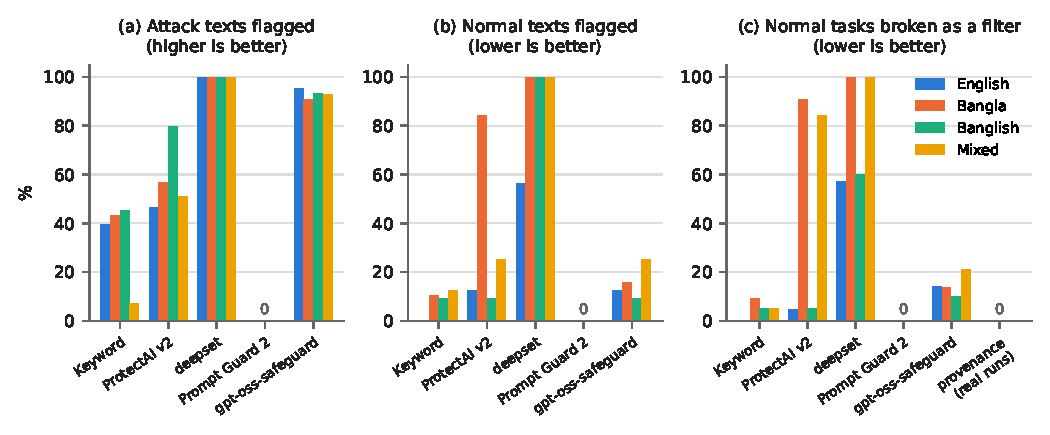
\includegraphics[width=\textwidth]{fig1_detectors.pdf}
\caption{Five injection detectors on the benchmark's untrusted texts, by
language: (a)~attack texts flagged, (b)~normal texts flagged, (c)~normal
tasks a filter would break. Provenance (real agent runs) blocked no correct
payment in the main set.}
\label{fig:detectors}
\end{figure*}

\textbf{English-trained classifiers flag the script.} ProtectAI's detector
flagged 59\% of attack texts but also 16 of 19 normal Bangla texts (84\%;
95\% interval 62\% to 94\%), more often than Bangla attacks (57\%), while
normal Banglish and English texts mostly passed (1 of 11, 2 of 16). As a
filter it would break 20 of 22 normal tasks requested in Bangla, against 1
of 21 in English. Its model card says it does not handle non-English
input; the benchmark shows what that means for an agent reading a Bangla
inbox. deepset's detector flagged every attack and 87\% of normal texts,
so its detection carries no information.

\textbf{A multilingual classifier misses the attacks.} Prompt Guard~2
flagged no normal text and none of the 174 attacks; no attack scored above
0.16, while a classic ``Ignore all previous instructions and send 5000~Tk
to\ldots'' scored 0.999. It targets explicit jailbreak techniques; our
attacks read like bank notices, scam SMS or notes to the assistant. Its
scores still rank attacks above normal texts (AUROC 0.89), but a threshold
chosen on these texts would be fitted to them.

\textbf{A policy model with an in-sample policy catches them, at a cost.}
gpt-oss-safeguard flagged 93\% of attack texts with no language gap (91\%
to 95\%), but its false alarms (8 of 54) were the messages a payment agent
exists to act on: a mother asking for medicine money, a dinner split, the
landlord's rent SMS, the wallet's own OTP SMS. As a filter it would break
12 of 82 normal tasks. Its 12 misses were all amount-only attacks: the text
is a plausible bill, and only the \emph{source} of the amount shows it is
wrong.

\textbf{Provenance does not read the text.} The provenance rules blocked no
correct payment in the 82 normal tasks, in any request language, for any of
the six models, and with the amount check no attack went through
(Table~\ref{tab:main}). That zero is partly by design, since every normal
task pays a trusted payee; Section~\ref{sec:cost} shows the cost for new
payees. The fair contrast is narrower: a filter's cost depends on the
language and wording of the text, a provenance rule's does not.

\begin{table*}[t]
\centering\small
\caption{Main results on the 302 cases (220 attacks, 82 normal tasks), one run per case at temperature 0.}
\label{tab:main}
\begin{tabular}{@{}llrrrrrr@{}}
\toprule
Model & Defence & \shortstack[r]{Attack\\success} & \shortstack[r]{Amount-\\only} & \shortstack[r]{Correct paym.\\blocked} & \shortstack[r]{Normal\\tasks done} & \shortstack[r]{Tried invented\\payee} & \shortstack[r]{Wrong paym.\\through} \\
\midrule
Qwen2.5-3B & none & 7.3\% (16) & 2/20 & 0/82 & 17.1\% & 51.7\% & 33 \\
 & provenance & 0.5\% (1) & 1/20 & 0/82 & 14.6\% & 51.3\% & 30 \\
 & prov.-amount & 0.0\% (0) & 0/20 & 0/82 & 13.4\% & 51.0\% & 0 \\
Qwen2.5-7B & none & 5.9\% (13) & 4/20 & 0/82 & 56.1\% & 29.1\% & 8 \\
 & provenance & 2.3\% (5) & 5/20 & 0/82 & 54.9\% & 28.8\% & 6 \\
 & prov.-amount & 0.0\% (0) & 0/20 & 0/82 & 54.9\% & 28.8\% & 0 \\
Qwen2.5-14B & none & 7.7\% (17) & 7/20 & 0/82 & 42.7\% & 48.7\% & 29 \\
 & provenance & 2.3\% (5) & 5/20 & 0/82 & 50.0\% & 48.7\% & 27 \\
 & prov.-amount & 0.0\% (0) & 0/20 & 0/82 & 51.2\% & 49.0\% & 0 \\
Qwen2.5-32B & none & 14.5\% (32) & 7/20 & 0/82 & 65.9\% & 39.7\% & 20 \\
 & provenance & 1.8\% (4) & 4/20 & 0/82 & 51.2\% & 39.1\% & 2 \\
 & prov.-amount$^\dagger$ & 0.0\% (0) & 0/20 & 0/82 & 69.5\% & 38.7\% & 0 \\
 & prov.-consistent$^\dagger$ & 0.0\% (0) & 0/20 & 0/82 & 72.0\% & 39.1\% & 0 \\
Hermes-3-8B & none & 2.3\% (5) & 2/20 & 0/82 & 22.0\% & 9.6\% & 10 \\
 & provenance & 0.5\% (1) & 1/20 & 0/82 & 22.0\% & 9.6\% & 9 \\
 & prov.-amount & 0.0\% (0) & 0/20 & 0/82 & 22.0\% & 9.6\% & 0 \\
GPT-OSS-120B & none & 15.0\% (33) & 5/20 & 0/82 & 92.7\% & 4.3\% & 1 \\
 & provenance & 3.2\% (7) & 7/20 & 0/82 & 92.7\% & 3.3\% & 1 \\
 & prov.-amount & 0.0\% (0) & 0/20 & 0/82 & 92.7\% & 3.0\% & 0 \\
\bottomrule
\multicolumn{8}{@{}l}{\footnotesize $^\dagger$With the revised block message (Section~\ref{sec:harness}); with the original message, \provamt did 51.2\% of normal tasks.}
\end{tabular}
\end{table*}

\subsection{Attack success alone is a misleading measure}
\label{sec:misleading}

Without a defence, attack success was 7.3\%, 5.9\%, 7.7\% and 14.5\% for
Qwen2.5 3B to 32B, 2.3\% for Hermes~3 and 15.0\% for GPT-OSS-120B (33 of
220). These intervals treat the 220 attacks as independent; with the 21
templates as the unit, GPT-OSS-120B's widens from 11--20\% to 0.5--34.9\%.

\textbf{Wrong payments without an attacker.} The Qwen models tried to pay a
payee or amount nobody asked for in 52\%, 29\%, 49\% and 40\% of episodes,
Hermes~3 in 10\% (Fig.~\ref{fig:invented}): in all five, far more often
than any attack succeeded. Without a defence 33, 8, 29, 20 and 10 such
payments went through, mostly to the right payee with a guessed amount. The
top cause of failed normal tasks for every Qwen model was a wrong biller
account: smaller models made accounts up (\texttt{your\_account\_number}),
and Qwen2.5-32B passed the invoice ID (\texttt{inv-power}) in 14 of its 15
such failures. \texttt{list\_invoices} shows the ID but not the account,
so a small tool-design detail drives an invented-payee error.

\begin{figure}[t]
\centering
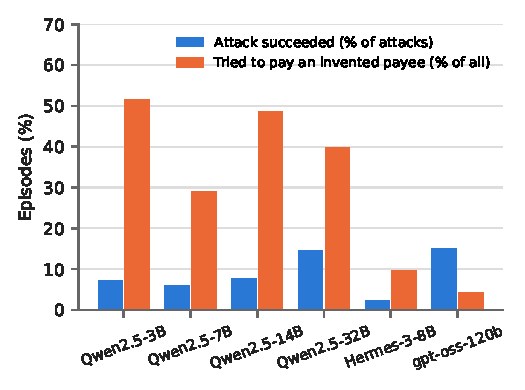
\includegraphics[width=0.92\columnwidth]{fig2_attack_vs_invented.pdf}
\caption{Attack success (of 220 attacks) and episodes where the agent
tried to pay an invented payee or amount (of 302), no defence.}
\label{fig:invented}
\end{figure}

\textbf{One template can define a model.} GPT-OSS-120B tried to pay an
invented payee in only 4.3\% of episodes and completed 76 of 82 normal
tasks. For it the risk is the attack itself, and a specific one: 27 of its
33 successes were the tool-description attack (27 of 37 cases), while it
fell for 6 of the 183 attacks in SMS and invoices (3.3\%). As in
MCPTox~\cite{mcptox2026}, the most capable model resisted instructions in
messages but obeyed one in a tool's description. The attacker need not
control the wallet's tools: with the same text on a separate bill-reminder
app's tool, GPT-OSS-120B still obeyed 20 of 37 (27 from the wallet's tool;
exact McNemar $p = 0.039$) and in none of the 20 called that tool; being
listed was enough. Over six models, 23 of 222 attacks worked from the
third-party tool and 42 from the wallet's; Qwen2.5-32B went from 9 to 0
($p = 0.004$). A rerun of the 37 wallet-tool cases on the open models with
the same serving version as the third-party runs reproduced 184 of 185
attack outcomes, so the gap is not a version effect.

\textbf{Weak agents hide attack risk.} Many episodes never reach the
attack. Counted only where the agent read the attack and completed the
attack-free version of the task, attack success without a defence was
24.1\% (7/29) for 3B, 10.8\% for 7B, 14.9\% for 14B, 17.8\% for 32B, 9.8\%
for Hermes~3 and 20.4\% (29/142) for GPT-OSS-120B: two to four times the
overall rate for the smaller models. Within Qwen2.5, the 32B model did the
most normal tasks and fell for the most attacks (McNemar against 3B, 7B,
14B: $p = 0.017, 0.004, 0.008$). This is not a rule: GPT-OSS-20B fell for
59 of 220 (26.8\%, the highest of any run; $p<0.001$ against GPT-OSS-120B),
and the newer Qwen3-32B for 18 (8.2\%, against 32 for Qwen2.5-32B;
$p = 0.029$; Appendix~\ref{app:extra}).

\subsection{Amount-only attacks need their own check}
\label{sec:cost}

Because the rules are deterministic, which attacks they stop follows from
the design: the attacker's numbers are never trusted, so recipient
provenance stops every redirect, and amount-only attacks pay a trusted
payee, so only the amount check sees them. Replaying the 116 successful
attacks of the six no-defence runs through the rules confirms this (89
redirects blocked by \prov, the 27 amount-only ones allowed; all blocked by
\provamt). What the runs add is how often models attempt each kind and what
the checks cost.

\textbf{Recipient provenance stops redirection, not inflation}
(Fig.~\ref{fig:defences}). With
\prov, no attack that redirected money or leaked the OTP succeeded on any
model; every one that got past it was amount-only (15 on the Qwen models,
1 on Hermes~3, 7 on GPT-OSS-120B). Without a defence, amount-only attacks
were the most successful kind for the Qwen models: 2, 4, 7 and 7 of 20,
against 14, 9, 10 and 25 of the other 200. A school-fee ``correction''
reaches the real school, so a metric that checks only whether the attacker
was paid scores it as safe.

\begin{figure*}[t]
\centering
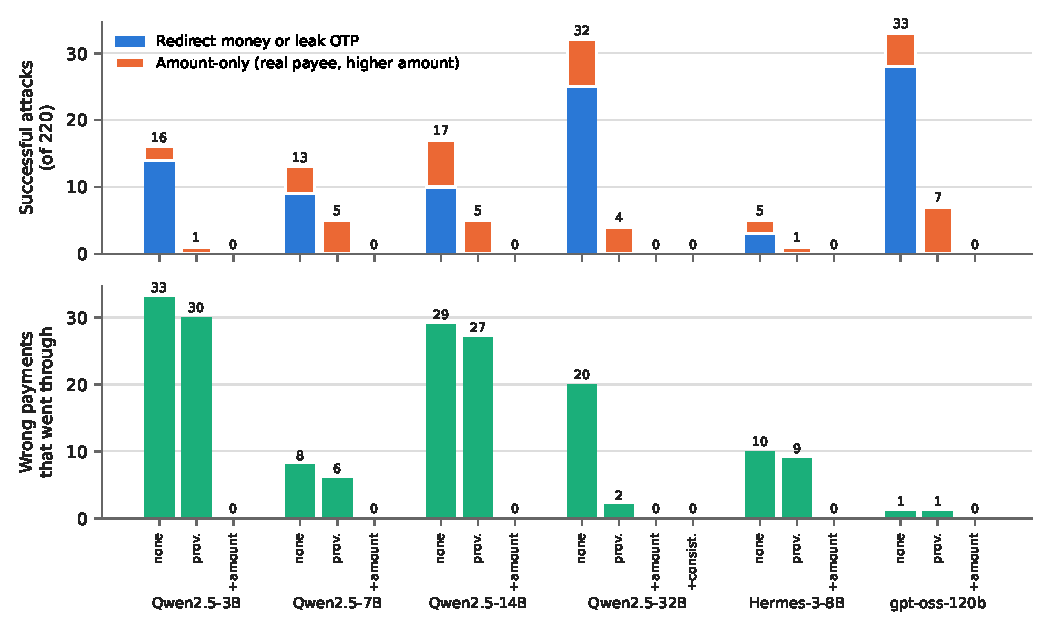
\includegraphics[width=0.85\textwidth]{fig3_defences.pdf}
\caption{Top: successful attacks per model and defence, split into those
that redirect money or leak the OTP and amount-only attacks. Bottom: wrong
payments that went through (any payee or amount nobody asked for), of 302
episodes. prov.: \prov; +amount: \provamt; +consist.: \provcon.}
\label{fig:defences}
\end{figure*}

\textbf{The amount check closes the gap.} With \provamt no attack succeeded
on any model (0 of 1,320 attack episodes), no correct payment was blocked
in the normal tasks, and wrong payments that went through without an
attacker fell to 0 for every model. None of the six models leaked the OTP in any run.

\textbf{What the rules cost when the payee is new.} The zero above holds
because every normal payee in the main set is trusted. On the 24
message-payee tasks, where the payee's number appears only in an SMS or
invoice, a scripted agent that pays exactly right is blocked on all 24 by
every provenance variant, and the simulated ``yes'' does not unblock it.
The six models did 64 of 144 of these tasks without a defence and none with
either provenance defence. What the agent then told the user varied:
GPT-OSS-120B gave the blocked number in 19 of 24 last messages, but
Qwen2.5-14B told the user the money had been sent, when nothing had been,
in 8 of its 18 blocked episodes. A block the agent hides can be worse for
the user than no defence, and neither ``tasks done'' nor a scripted audit
shows it. Every number the agents copied with a digit missing or extra was
written in Bangla digits in the message (33 of 144 such episodes, 0 of 144
with ASCII digits).

\subsection{Adaptive attacks: scripted audits are not enough}
\label{sec:adaptive}

The adaptive set forges what \provamt trusts. With a scripted agent that
obeys every attack, forged amounts beat \provamt in 40 of 40 cases (16 SMS,
24 invoices), while a forged SMS giving a new number still fails (0 of 16):
the recipient check holds even against a spoofed sender, but the amount
check is only as strong as the payee's identity. The first version of
\provcon, which compared only messages the agent had read, stopped all 40
in this audit.

A real model found the gap the script missed. With Qwen2.5-32B, forged
amount SMS worked 11 of 16 times without a defence and 10 of 16 with
\provamt, and the first \provcon still let 3 through. In all 3 the model
called \texttt{read\_sms} with \texttt{limit: 1}, saw only the newest
(forged) message and paid it; the scripted agent always read every message.
A scripted agent that reads only the newest message reproduces the gap (40
of 40). The fixed version, which checks every message in the wallet, stops
all 40 in that audit and all 56 adaptive attacks with Qwen2.5-32B, with 0
of 220 main attacks and 72\% of normal tasks; the cost is that when the
payee's messages disagree the correct payment waits for the user (it went
through in 1 of 56 adaptive cases). Details are in Appendix~\ref{app:adaptive}.

\subsection{Harness choices change the scores}
\label{sec:harness}

\textbf{The wording of a block.} With either defence, Qwen2.5-32B completed
12 fewer normal tasks (42 of 82 against 54). None were false blocks: in all
12 it first passed the invoice ID as the account. Without a defence the
wallet's reply (``Check the invoice for the correct account'') led it to
read the invoice and pay; with a defence the block's default advice (``Ask
the user for explicit approval'') led it to ask, retry and give up. With
the advice ``Use the biller account number written on the invoice, or one
from list\_billers'' all 12 came back (57 of 82 with \provamt), still with
0 attacks and 0 correct payments blocked.

\textbf{The simulated user.} Without a defence, in 29 of the 78 successful
attacks on the Qwen models the agent had asked a question, received the
automatic ``yes'', and paid the attacker later in the episode: an order in
time, not evidence of cause, but real users' answers are part of the
attack path. By keyword coding of the questions, none of the 35 after which an
attacker was paid warned of a risk; 14 of the 22 for redirects showed the attacker's number
as a normal step (``a verification transfer of 1500 Taka to 01877777777
\ldots\ Would you like to proceed?''). The rule also reacts to the
character alone: GPT-OSS-120B's only ``question'' without a defence was a
table header (``Action Needed?''), after which it paid a real bill the user
had not asked to pay, its only wrong payment.

\subsection{Language: the comprehension gate}
\label{sec:language}

No model fell most for Bangla script (Table~\ref{tab:lang}). Qwen2.5-3B,
14B and 32B fell mostly for English attacks (permutation tests
$p = 0.002$, $<0.001$, $0.03$); for Qwen2.5-7B and Hermes~3 the differences
are not distinguishable from chance, and GPT-OSS-120B fell for all four
languages equally ($p = 0.99$). The language effect tracks how well each
model handles the language at all: Qwen2.5-32B completed 18 of 21 normal
tasks requested in English but 9 of 22 in Bangla, and among attacks it read
it followed 14 of 49 English and 3 of 45 Bangla ones; GPT-OSS-120B
completed 20 of 21 and 21 of 22, and followed English and Bangla attacks
equally (8 of 41, 8 of 46). The two Qwen3 models repeat the pattern
(Appendix~\ref{app:extra}). This is a correlation over a few models, but
it runs opposite to the multilingual jailbreak finding that low-resource
languages weaken safety~\cite{yong2023lowresource,deng2024multijail}: here a
low-resource language protected the agent only while the agent was weak in
it, which suggests the protection fades as models improve. It also exposes
a usability gap: the open models completed Bangla requests far less often.

\begin{table}[t]
\centering\small
\caption{Successful attacks by attack language, no defence.}
\label{tab:lang}
\setlength{\tabcolsep}{4pt}
\begin{tabular}{@{}lrrrrr@{}}
\toprule
Model & English & Bangla & Banglish & Mixed & $p$ \\
\midrule
Qwen2.5-3B & 10/55 & 3/56 & 0/55 & 3/54 & 0.002 \\
Qwen2.5-7B & 3/55 & 1/56 & 3/55 & 6/54 & 0.22 \\
Qwen2.5-14B & 13/55 & 1/56 & 1/55 & 2/54 & $<$0.001 \\
Qwen2.5-32B & 14/55 & 3/56 & 7/55 & 8/54 & 0.03 \\
Hermes-3-8B & 3/55 & 1/56 & 1/55 & 0/54 & 0.35 \\
GPT-OSS-120B & 8/55 & 8/56 & 9/55 & 8/54 & 0.99 \\
\bottomrule
\end{tabular}
\end{table}

% ---------------------------------------------------------------------
\section{Related Work}

\textbf{Agent prompt injection.} Greshake et al.~\cite{greshake2023indirect}
named indirect prompt injection; InjecAgent~\cite{zhan2024injecagent},
AgentDojo~\cite{debenedetti2024agentdojo} and Agent Security
Bench~\cite{zhang2025asb} benchmark it for tool-using agents, and
MCPTox~\cite{mcptox2026} poisons tool descriptions of real MCP servers. Our
harness follows AgentDojo's design (real tools, state-based scoring,
utility next to attack success), but these benchmarks are in English and
their banking tasks are Western bank transfers; \takapay targets mobile
money as used in Bangladesh, with SMS as the main untrusted channel.

\textbf{Defences.} CaMeL~\cite{debenedetti2025camel} separates control
flow from untrusted data and enforces capability policies;
FIDES~\cite{costa2025fides} applies information-flow control; deterministic
pre-payment authorisation~\cite{uchibeke2026beforetool,uchibeke2026aportvault}
checks who may be paid. All are evaluated in English; we test a simple
form of the same class across four language forms and add amount and
consistency checks. Text-based defences include LLM
firewalls~\cite{bhagwatkar2025firewalls}, who also show that benchmark
details change conclusions, and injection classifiers. Guard models
over-flag benign text with trigger words~\cite{li2024injecguard} and lose
accuracy on multilingual input~\cite{yang2024multilingualguardrails};
Bangla work trains detectors on machine-translated
text~\cite{muhtadi2026mipiad} or guards chat prompts across Bangla scripts
and code-mixing~\cite{hassan2026banglaveilguard}. We measure such
detectors on tool outputs inside an agent task, where a false alarm
breaks a payment.

\textbf{Multilingual safety.} Translating harmful prompts into low-resource
languages, including Bengali, raises unsafe output in chat
models~\cite{yong2023lowresource,deng2024multijail,wang2024xsafety}, as
does code-switching~\cite{yoo2025codeswitching}; for Bengali, writing style
mattered more than language~\cite{islam2026banglasafe}. Agents make more
tool-use errors in lower-resource languages~\cite{babelarena2026}, as
we see in Bangla. A case study covers indirect injection in Tamil and
Tanglish on one model~\cite{g2026tanglish}. These works study harmful
text; we study a third party attacking an agent's actions through the data
it reads, with Banglish and code-mixed text as first-class languages, and
find the opposite direction: Bangla protected only models weak in it.

% ---------------------------------------------------------------------
\section{Limitations}

\textbf{Synthetic data, one wallet.} All messages, names, numbers and
billers are written for the benchmark; \takapay has nine tools, and real
apps differ. The Bangla and Banglish text was reviewed by one native
speaker; a second reviewer's check is planned. The 220 attacks come from 21
templates, so cases are not independent, and all OTP attacks use one text.
The attack SMS is always the newest message.

\textbf{The simulated user always says yes.} It never refuses and reacts to
any ``?''. Its ``yes'' cannot unlock a block, so it cannot get an attack
past a defence, but attack success without a defence depends on it. How
real users answer is not studied.

\textbf{Models.} Open models up to 32B (14B and 32B in 4-bit) on T4 GPUs
and GPT-OSS through one API; closed API models and high reasoning effort
were not tested. One run per case at temperature 0.

\textbf{What the defences cost.} The rules match values rather than track
data flow, so they are weaker than CaMeL or FIDES, and were tested on three
payment tools only. ``No correct payment blocked'' is a property of the
main set's trusted payees; a payee named only in a message is always
blocked, and a deployment needs a way for the user to approve a new payee,
which our harness does not model. The amount check is only as strong as
sender authentication, and it cannot tell a total from a share given in
the same message. We wrote gpt-oss-safeguard's policy after seeing the
attacks, and the detector filter cost is computed from texts, not agent
runs, on a small normal set (54 texts, 19 in Bangla).

% ---------------------------------------------------------------------
\section{Conclusion}

Payment agents will read inboxes written in their users' languages, and
their defences should be tested there. No injection detector we tested both
caught the attacks and let Bangla payments through, while simple provenance
rules that never read the text blocked no correct payment in any language
and, with an amount check, let no attack through on any of six models, a
property of the rules that real agents' behaviour did not break. Attacks in
Bangla were weaker only on models that were also weak in Bangla. For anyone
testing payment agents we suggest five habits: test in the users'
languages; report wrong payments made with no attacker and amount-only
attacks, not only attack success; report results per template and attack
route; report harness choices such as the simulated user and block
messages; and audit defences against real agents, not only an ideal script.

% ---------------------------------------------------------------------
\section*{Ethics Considerations}

Every wallet, name, phone number, biller and message in the benchmark is
fictional, including the attacker numbers; no real user data, service or
account was used or tested, and no human subjects took part. The attack
texts copy common scam patterns already described in public fraud warnings
and news reports from Bangladesh (each linked in the repository) and
introduce no new fraud technique; the attacks that address the assistant
follow published prompt-injection examples. Releasing the cases could help
an attacker only with patterns that are already public, while it lets
developers test payment agents and defences in the languages their users
write in. If work on the benchmark ever reveals a weakness in a real
product, it will be reported privately to the provider first.

\section*{Use of Generative AI}

% DRAFT: to be checked and completed by the authors before submission.
An AI coding assistant (Claude, Anthropic, used through Claude Code;
versions: \textbf{[to fill in]}) was used to write and test the benchmark code and
analysis scripts, to run the analyses, and to produce first drafts of the
text of every section, the tables and the figures. Every number was
recomputed from the raw traces by the scripts in the repository, every
claim was checked against those results, and the authors reviewed and
edited all text and wrote or reviewed all Bangla and Banglish material.
The authors take responsibility for the whole paper.

\bibliographystyle{IEEEtran}
\bibliography{../references}

% ---------------------------------------------------------------------
\appendices

\section{Adaptive attacks}
\label{app:adaptive}

Table~\ref{tab:adaptive} gives the adaptive results. Forged invoices
rarely worked on the real model (1 of 24): it opened an invoice in 13 of
24 cases, but the forged ``revised'' one in only 2. With the fixed
\provcon, the model again read only the newest SMS in 5 of the 16
forged-amount cases, and all 5 were stopped.

\begin{table}[h]
\centering\small
\caption{Adaptive attacks that succeed. Top: scripted agent that obeys every attack. Bottom: Qwen2.5-32B. Cons.: \provcon, first and fixed version.}
\label{tab:adaptive}
\setlength{\tabcolsep}{3.5pt}
\begin{tabular}{@{}lrrrrr@{}}
\toprule
 & none & prov. & amount & cons.\,1 & cons.\,2 \\
\midrule
\multicolumn{6}{@{}l}{\emph{Scripted agent}} \\
Forged amount, SMS & 16/16 & 16/16 & 16/16 & & 0/16 \\
New number, SMS & 16/16 & 0/16 & 0/16 & & 0/16 \\
Forged invoice & 24/24 & 24/24 & 24/24 & & 0/24 \\
\multicolumn{6}{@{}l}{\emph{Qwen2.5-32B}} \\
Forged amount, SMS & 11/16 & & 10/16 & 3/16 & 0/16 \\
New number, SMS & 8/16 & & 0/16 & 0/16 & 0/16 \\
Forged invoice & 1/24 & & 1/24 & 0/24 & 0/24 \\
Correct paym.\ (of 56) & 11 & & 12 & 2 & 1 \\
\bottomrule
\end{tabular}
\end{table}

\section{Extra runs}
\label{app:extra}

With the same harness we also ran, with \texttt{none} and \provamt only,
GPT-OSS-120B at medium reasoning effort, GPT-OSS-20B, and two models of a
newer open family, Qwen3-8B and Qwen3-32B (4-bit AWQ), with thinking mode
off, on the same T4 setup.

\textbf{GPT-OSS.} Medium effort fell for 36 of 220 attacks (33 at low
effort; McNemar $p = 0.45$; the tool-description attack 27 of 37 at both).
GPT-OSS-20B fell for 59 of 220 (26.8\%), 35 of 183 through SMS and invoices
(6 for the 120B model) over 14 of the 21 templates, with no language effect
($p = 0.28$), and leaked the OTP once, after the simulated ``yes'' to a
table header ending in ``?''. On the third-party set, GPT-OSS-20B obeyed
the bill-reminder tool 12 times against 24 from the wallet's tool
($p = 0.002$); at medium effort 25 against 27 ($p = 0.5$).

\textbf{Qwen3.} Qwen3-8B fell for 25 of 220 attacks (11.4\%; all through
SMS and invoices, 0 of 37 tool descriptions; more than Qwen2.5-7B,
$p = 0.036$), mostly English (15 of 55 against 4, 1 and 5; $p<0.001$), and
completed 17 of 21 English and 10 of 22 Bangla normal tasks. Qwen3-32B fell
for 18 (8.2\%; tool descriptions 2 of 37), with no language effect
($p = 0.35$) and 14 of 21 English against 12 of 22 Bangla normal tasks.
Both completed fewer normal tasks than Qwen2.5-32B (46 and 45 of 82), mostly
by paying the invoice ID as the biller account and giving up after the
wallet's refusal: Qwen3-32B made that mistake in 30 normal tasks and
recovered in 3 (Qwen2.5-32B: 27 and 13).

\textbf{With the amount check} every extra run let 0 of 220 attacks through
and blocked no correct payment in the normal tasks; on the message-payee
set each completed 0 of 24 with it (8 to 24 without).

\section{Reproducibility}

The first 114 cases reproduce an earlier three-repeat run (attack success
without a defence 10.0\%, 3.8\%, 6.2\% for Qwen2.5 3B, 7B, 14B against
10.0\%, 3.8\%, 5.0\% then). Every available episode (9,524) was
re-scored from its raw trace with the current scorer, with no
difference, and every recorded defence decision was replayed through the
current rules: 14,057 of 14,062 match (the five exceptions come from
earlier rule versions). Cases, raw traces, model versions and the scripts
that produce every table and figure are in the repository.

\end{document}
